\subsection{勾股定理}\label{subsec:czjh1-5-3}

如图 \ref{fig:czjh1-5-14}, 我们把两个全等的正方形,用对角线分成四个全等的等腰直角三角形,然后把它们拼成一个正方形。
这个正方形的边,恰好是以前两个正方形的边为腰的等腰直角三角形的斜边。
因此,等腰直角三角形两腰上的正方形面积的和,等于斜边上正方形的面积。
我们可以证明,对于一般的直角三角形也有这种关系(图 \ref{fig:czjh1-5-15})。
由于正方形的面积等于它的一边的平方,这种关系可写成下面定理:

\begin{figure}[htbp]
    \centering
    \begin{minipage}[b]{7cm}
        \centering
        \begin{tikzpicture}
    \pgfmathsetmacro{\a}{2}
    \tkzDefPoints{0/0/A, \a/0/B, \a/\a/C, 0/\a/D, 0/\a+\a/E, \a/\a+\a/F}
    \tkzInterLL(D,F)(C,E)  \tkzGetPoint{O}
    \tkzDefTriangle[two angles=45 and 45](D,E)  \tkzGetPoint{G}
    \tkzDefTriangle[two angles=45 and 45](F,C)  \tkzGetPoint{H}

    \tkzDrawPolygon(A,B,C,D)
    \tkzDrawPolygon(D,G,E,O)
    \tkzDrawPolygon(C,H,F,O)
    \tkzDrawSegments[dashed](A,C  B,D  D,E  C,F)
\end{tikzpicture}


        \caption{}\label{fig:czjh1-5-14}
    \end{minipage}
    \qquad
    \begin{minipage}[b]{7cm}
        \centering
        \begin{tikzpicture}[scale=0.4]
    \pgfmathsetmacro{\a}{4}
    \pgfmathsetmacro{\b}{3}
    \pgfmathsetmacro{\c}{5}

    \tkzDefPoints{0/0/A,  \c/0/B}
    \tkzInterCC[R](A,\b)(B,\a)  \tkzGetFirstPoint{C}
    \tkzLabelPoints[above=.5em](C)
    \tkzLabelPoints[below left](A)
    \tkzLabelPoints[right](B)
    \tkzLabelSegment[above right](B,C){$a$}
    \tkzLabelSegment[above left](A,C){$b$}
    \tkzLabelSegment[below](A,B){$c$}
    % \tkzDrawPolygon(A,B,C)

    \tkzDefSquare(B,A)
    \tkzDrawPolygon(B,A,tkzFirstPointResult,tkzSecondPointResult)

    \tkzDefSquare(A,C)
    \tkzDrawPolygon(A,C,tkzFirstPointResult,tkzSecondPointResult)

    \tkzDefSquare(C,B)
    \tkzDrawPolygon(C,B,tkzFirstPointResult,tkzSecondPointResult)
\end{tikzpicture}


        \caption{}\label{fig:czjh1-5-15}
    \end{minipage}
\end{figure}

\begin{dingli}[定理]
    直角三角形两直角边 $a$、$b$ 的平方和,等于斜边 $c$ 的平方。
\end{dingli}

\begin{center}
    \framebox[10em]{\zhongdian{
        $\bm{a^2 + b^2 = c^2}$。
    }}
\end{center}

已知:在 $Rt \triangle ABC$ 中,$AB = c$, $BC = a$, $CA = b$(图 \ref{fig:czjh1-5-16} 甲)。

求证:$a^2 + b^2 = c^2$。

\zhengming 如图 \ref{fig:czjh1-5-16} 乙那样, 取四个与 $Rt \triangle ABC$ 全等的三角形,放在边长为 $a + b$ 的正方形内,
得到边长分别为 $a$、$b$ 的正方形 I、 II。

再将同样的四个直角三角形,如图 \ref{fig:czjh1-5-16} 丙那样放在边长为 $a + b$ 的正方形内,这时,
得到的四边形 III 也是正方形,并边长等于 $\triangle ABC$ 的斜边 $c$。

\begin{figure}[htbp]
    \centering
    \begin{minipage}[b]{3cm}
        \centering
        \begin{tikzpicture}
    \pgfmathsetmacro{\factor}{0.5}
    \pgfmathsetmacro{\a}{4 * \factor}
    \pgfmathsetmacro{\b}{3 * \factor}
    \pgfmathsetmacro{\c}{5 * \factor}

    \tkzDefPoints{0/0/C, \b/0/A, 0/\a/B}

    \tkzDrawPolygon(A,B,C)
    \tkzLabelPoints[above](B)
    \tkzLabelPoints[left](C)
    \tkzLabelPoints[right](A)
    \tkzLabelSegment[below](C,A){$b$}
    \tkzLabelSegment[left](C,B){$a$}
    \tkzLabelSegment[right](A,B){$c$}
\end{tikzpicture}


        \caption*{甲}
    \end{minipage}
    \qquad
    \begin{minipage}[b]{5cm}
        \centering
        \begin{tikzpicture}
    \pgfmathsetmacro{\factor}{0.5}
    \pgfmathsetmacro{\a}{4 * \factor}
    \pgfmathsetmacro{\b}{3 * \factor}
    \pgfmathsetmacro{\c}{5 * \factor}

    \tkzDefPoints{0/0/A, \a+\b/0/B, \a+\b/\a+\b/C, 0/\a+\b/D}
    \tkzDefPoints{\a/0/E, \a+\b/\a/F, \a/\a+\b/G, 0/\a/H}
    \tkzInterLL(E,G)(F,H)  \tkzGetPoint{O}

    \tkzDrawPolygon(A,B,C,D)
    \tkzFillPolygon[gray!20](D,H,O,G)
    \tkzFillPolygon[gray!20](E,B,F,O)
    \tkzDrawSegments(E,G  F,H  D,O  B,O)

    \tkzLabelSegment[above](D,G){$a$}
    \tkzLabelSegment[above](G,C){$b$}
    \tkzLabelSegment[left](A,H){$a$}
    \tkzLabelSegment[left](H,D){$b$}

    \tkzLabelSegment(A,O){I}
    \tkzLabelSegment(O,C){II}
\end{tikzpicture}


        \caption*{乙}
    \end{minipage}
    \qquad
    \begin{minipage}[b]{5cm}
        \centering
        \begin{tikzpicture}
    \pgfmathsetmacro{\factor}{0.5}
    \pgfmathsetmacro{\a}{4 * \factor}
    \pgfmathsetmacro{\b}{3 * \factor}
    \pgfmathsetmacro{\c}{5 * \factor}

    \tkzDefPoints{0/0/A, \a+\b/0/B, \a+\b/\a+\b/C, 0/\a+\b/D}
    \tkzDefPoints{\b/0/E, \a+\b/\b/F, \a/\a+\b/G, 0/\a/H}
    \tkzInterLL(E,G)(F,H)  \tkzGetPoint{O}

    \tkzDrawPolygon(A,B,C,D)
    \tkzDrawPolygon[fill=gray!20](H,A,E)
    \tkzDrawPolygon[fill=gray!20](E,B,F)
    \tkzDrawPolygon[fill=gray!20](F,C,G)
    \tkzDrawPolygon[fill=gray!20](G,D,H)

    \tkzLabelSegment[above](D,G){$a$}
    \tkzLabelSegment[above](G,C){$b$}
    \tkzLabelSegment[left](A,H){$a$}
    \tkzLabelSegment[left](H,D){$b$}
    \tkzLabelSegment[below](G,H){$c$}

    \tkzLabelSegment(A,C){III}
\end{tikzpicture}


        \caption*{丙}
    \end{minipage}
    \caption{}\label{fig:czjh1-5-16}
\end{figure}


比较乙、丙两个图形,正方形 I、II 的面积的和 $a^2 + b^2$ 与正方形 III 的面积 $c^2$
都是同一正方形面积与 4 倍 $\triangle ABC$ 面积的差,所以
\begin{gather*}
    a^2 + b^2 = c^2 \juhao
\end{gather*}

这个定理的逆命题也成立。

\begin{dingli}[逆定理]
    如果三角形的三边长 $a$、$b$、$c$ 有下面关系:
    \begin{gather*}
        a^2 + b^2 = c^2 \douhao
    \end{gather*}
    那么这个三角形是直角三角形。
\end{dingli}

已知: 在 $\triangle ABC$ 中,$AB = c$, $BC = a$, $CA = b$, 并且 $a^2 + b^2 = c^2$ (图 \ref{fig:czjh1-5-17})。

求证: $\angle C = Rt \angle$。

\begin{figure}[htbp]
    \centering
    \begin{tikzpicture}
    \pgfmathsetmacro{\factor}{0.5}
    \pgfmathsetmacro{\a}{3 * \factor}
    \pgfmathsetmacro{\b}{4 * \factor}
    \pgfmathsetmacro{\c}{5 * \factor}

    \begin{scope}
        \tkzDefPoints{0/0/B, \a/0/C, \a/\b/A}

        \tkzDrawPolygon(A,B,C)
        \tkzLabelPoints[above](A)
        \tkzLabelPoints[left](B)
        \tkzLabelPoints[right](C)
        \tkzLabelSegment[right](C,A){$b$}
        \tkzLabelSegment[below](C,B){$a$}
        \tkzLabelSegment[left](A,B){$c$}
    \end{scope}

    \begin{scope}[xshift=4cm]
        \tkzDefPoints{0/0/B', \a/0/C', \a/\b/A'}

        \tkzDrawPolygon[dashed](A',B',C')
        \tkzLabelPoints[above](A')
        \tkzLabelPoints[left](B')
        \tkzLabelPoints[right](C')
        \tkzLabelSegment[right](C',A'){$b$}
        \tkzLabelSegment[below](C',B'){$a$}
        \tkzLabelSegment[left](A',B'){$c$}
        \tkzMarkRightAngle(A',C',B')
    \end{scope}
\end{tikzpicture}


    \caption{}\label{fig:czjh1-5-17}
\end{figure}

\zhengming 作 $\triangle A'B'C'$, 使 $\angle C' = Rt \angle$, $B'C' = a$, $C'A' = b$, 那么

\qquad $A'B'^2 = a^2 + b^2$。

\begin{tblr}{colsep=0pt}
    $\because$ \quad  $a^2 + b^2 = c^2$, & $\therefore$ \quad $A'B'^2 = c^2$。 \\
    $\because$ \quad 边长是正值, \qquad   & $\therefore$ \quad $A'B' = c$。
\end{tblr}

在 $\triangle ABC$ 和 $\triangle A'B'C'$ 中,

$\because$ \quad \begin{zmtblr}[t]{}
    $BC = a = B'C'$, \\
    $CA = b = C'A'$, \\
    $AB = c = A'B'$, \\
\end{zmtblr}

$\therefore$ \quad $\triangle ABC \quandeng \triangle A'B'C'$。

$\therefore$ \quad $\angle C = \angle C' = Rt \angle$。

例如, $3^2 + 4^2 = 5^2$, $5^2 + 12^2 = 13^2$,…,
所以,边长分别是 3、4、5; 5、12、13; … 的三角形都是直角三角形。

在我国古代,一部数学书《周髀算经》中有用边为 3、4、5 的直角三角形来进行测量的记载,
并把直角三角形的两直角边分别叫做\zhongdian{勾}和\zhongdian{股},斜边叫做\zhongdian{弦}。
因此,我们把上面两个定理分别叫做\zhongdian{勾股定理}和它的逆定理。
勾股定理是数学中最常用的定理之一。
在外国是古希腊人毕达哥拉斯首先发现这个定理的,所以把它叫做\zhongdian{毕达哥拉斯定理}。


\begin{lianxi}

\xiaoti{在 $Rt \triangle ABC$ 中,$\angle C = Rt \angle$。}
\begin{xiaoxiaotis}

    \xxt{已知 $a = 6$, $b = 8$, 求 $c$;}

    \xxt{已知 $a = 40$, $c = 41$, 求 $b$。}

\end{xiaoxiaotis}


\xiaoti{边长为
    (1) $a = 8$, $b = 15$, $c = 17$;
    (2) $a = 7$, $b = 24$, $c = 25$
    的三角形是不是直角三角形?是直角三角形的,哪个角是直角?
}

\xiaoti{正三角形的边长为 $10 \;\limi$, 求这个三角形的面积。}

\end{lianxi}

